\chapter{理論}
\section{AIを用いた楽曲作成}
\subsection{MIDI}
AIによる曲制作では主にMIDIファイルの音楽データを使用する.MIDI ファイルには実際の音ではなく音楽の演奏情報(音の高さや長さなど)である.
本研究で用いるAIはこのMIDIファイルの情報を元に学習をする.また入出力の際もこの規格を用いる.
\subsection{Magenta}
本研究ではMagenta[1]を使用する.これは音楽などをTensorFlowを使って機械学習するライブラリであり,Google BrainがGitHab上に公開している.
Magentaではまず学習させたい音楽のMIDIデータをファイルに格納しNoteSequence(magentaが扱うファイル形式)に変更する.それを学習用データセットに変換したあと学習を行う.このとき,一度に学習させるデータの数,学習を行う回数,ノード数を設定する.これをパッケージ化し,MIDIファイルとして新たに楽曲を生成するという流れである.これを図2.1に示す.\\
\newpage
\begin{figure}[!ht]
    \begin{screen}
    \begin{center}
        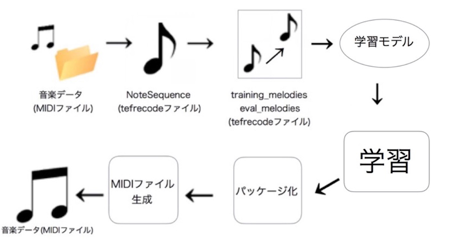
\includegraphics[scale=1.5, clip]{./img/magenta_usestep.png}
        \caption{magentaによるMIDI音楽データ生成までのプロセス}
        \label{fig:magentaによるMIDI音楽データ生成までのプロセス}
    \end{center}
    \end{screen}
    \end{figure}
\begin{itemize}
\section{開発環境の構築}
開発環境の構築にはコンテナ型仮想環境を提供するオープンソフトウェアであるDockerを用いた.\\
 Dockerには仮想環境を配布可能な形にする事ができるDockerImageがあり,そのImageを用いる事で同一の実行環境が作成できる.
また,クラウド上でDockerImageを配布できるDockerHubというサービスがあり,そのサービス上にすでにMagentaの開発環境を構築済みの仮想環境があるため、その環境を今回は利用した.